\section{Experimental Setup and Results}
\label{sec: experimental-setup-and-results}
This chapter presents our deployment setup, the methodology used for performance measurement, and the results obtained under a range of different experimental scenarios.

\subsection{Deployment and Metrics Collection}
\label{subsec: deplyment-and-metrics-collection}
We conducted all experiments on a dedicated 4-node high-performance cluster located in our university. Each node is equipped with dual AMD EPYC 7H12 processors (resulting in 256 hardware threads) and 503 GiB of RAM. The nodes are interconnected via 10 Gigabit Ethernet.

In our experiments, we simulated a geo-distributed deployment by using all four physical nodes and injecting artificial network latency between them. Both clients and servers are deployed as Docker containers to ensure a clean and reproducible environment. The Figure~\ref{fig: overall-architecture} illustrates the setup. The data is divided into two partitions and fully replicated across two different regions. So, each region consists of two server containers that hold a complete copy of both partitions.  Unless stated otherwise, the clients are uniformly distributed across the two regions, and the number of client containers is varied between experiments to test scalability. By default, intra-region communication takes 0.5 ms round-trip time (RTT), while inter-region communication takes 50 ms.

For performance evaluation, each client container collects local metrics during execution, which are then aggregated by a centralized admin. The metrics we focus on are throughput, latency, abort rates, and bytes transferred, and we also estimate the operational cost. Throughput and abort rates are measured directly by the application logic, while latency and bytes transferred are collected using system-level network monitoring tools. Additionally, we estimate the cost by monitoring the resource utilization within the server containers and tracking the overall network usage.  

\subsection{Evaluation Scenarios and Results}
\label{subsec: evaluation-scenarios-and-results}
We now describe the experimental scenarios used in our evaluation. We designed these scenarios to systematically observe the impact of different system configurations on the transactional performance of the database systems. Each scenario is strongly connected with the tunable parameters shown in Figure~\ref{fig: overall-architecture}, which control the network conditions, the clients' placement, and the transactional load.

\subsubsection{Baseline Scenario}
\subsubsection{Skewed Access Scenario}
\subsubsection{Sunflower Topology Scenario}
\subsubsection{Scalability Scenario}
\subsubsection{Network Delays Scenario}
\subsubsection{Packet Loss Scenario}

\begin{figure*}[ht]
    \centering
    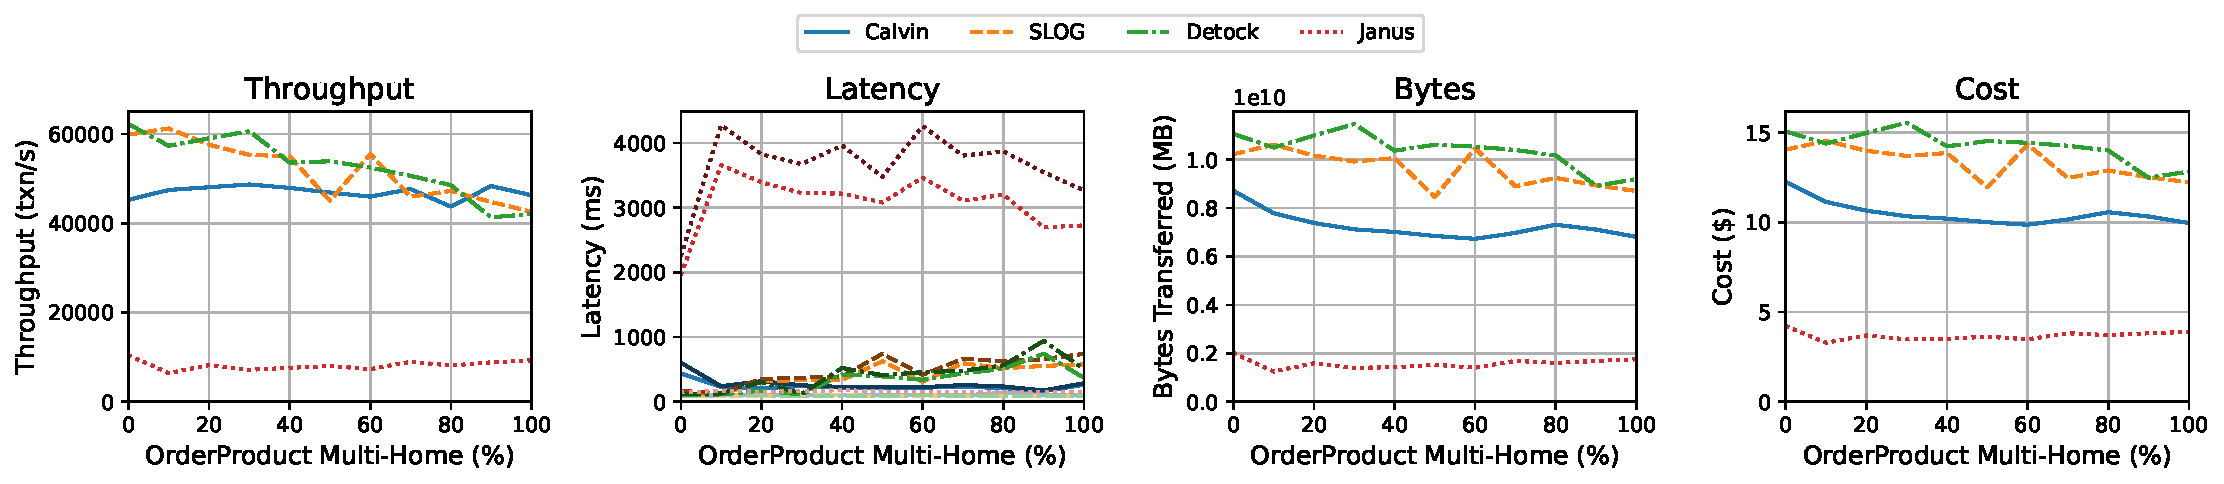
\includegraphics[width=1\textwidth]{figures/Baseline.pdf}
    \caption{Baseline Scenario Results.}
    \label{fig: baseline-scenario}
\end{figure*}

\begin{itemize}
    \item Describe cluster setup and the deployment configurations.
    \item Explain the different scenarios that will be tested and how they will be tested.
    \item Present raw data (latency, throughput, abort rate, byte transfers, resource demands).
\end{itemize}